% Angular, Mongoose MongoDB
%Client Webanwendungen, single page application Bootstrap
%Zentralisierung der Daten (Sicherheit)
%Android debug bridge ADB


\chapter{Technischen Grundlagen} \label{Theoretische Grundlagen}
Im diesem Kapitel werden die Technischen Grundlagen der verwendeten Technologien im einzelnen betrachtet.

\section{Daten beim Aufrufen oder Wechseln einer Seite übergeben}
Bei Webanwendungen, wie die im Rahmen dieser Arbeit entstandenen, ist es immer wieder nötig zum Beispiel beim Wechsel zu einer anderen Seite Daten an diese zu übergeben. Dies kann auf verschiedenen Wegen geschehen.

Bei kleiner Datenmengen wie Beispielsweise einer Id wird diese meinst in der URL übergeben. Diese wird dann an die eigentlich aufzurufende URL (z.B. http://eine.ip/index.html) nach einem \textbf{"< ? ">} angehängt.
Die aufzurufende URL hat dann Beispielsweise die Form \\ \textit{http://eine.ip/index.html?patientId=eine1Id}.
Wird die Seite auf diese Art aufgerufen, kann die Variable \textbf{patientId} dann von dieser ausgelesen werden. Soll mehr wie eine Variable übergeben werden,können diese mit dem \textbf{"< \& ">} Zeichen aneinander angehängt werden.

Wenn größere Datenmengen zu übertragen sind, werden diese innerhalb des HTTP Objektes in dessen Rumpf übergeben. Dies wird in dieser Anwendung Beispielsweise verwendet, wenn nach der Anfrage an den Datenbank Server dessen Antwort mit dem Objekt im JSON Format Beispielsweise eines Patienten zurück gesendet wird.

\section{REST-Service}
Um eine gemeinsame Datenbasis zwischen den beiden Clients für Therapeut und Patient zu schaffen bietet der im Rahmen dieser Arbeit entwickelte Server einen REST-Service zum abrufen der in der Datenbank gespeicherten Daten an. Mit dessen Hilfe können die Daten zu den Patienten, Aufgaben und Fragebögen über das Internet mittels HTTP Anfragen auf jedem Gerät abgerufen und verändert werden. Das Programmierparadigma eines REST-Services soll dabei verschiedenen Prinzipien folgen.

Zum einen soll dieser Service \textbf{zustandslos} sein. Bei jedem Aufruf müssen somit alle zum verstehen der Nachricht nötigen Daten übermittelt werden.
Ein weiteres Prinzip ist die \textbf{Adressierbarkeit} der einzelnen Ressourcen, welches in dieser Anwendung durch die einzigartige Id jedes Objekts realisiert wurde.
\subsection{Die HTTP-Methoden}
Um mit dem Service zu interagieren stehen verschiedene HTTP-Methoden zu Verfügung. Welche hier kurz erklärt werden.
\paragraph{HTTP-GET}
Mittels HTTP-GET wird dem Server signalisiert, dass Daten abgerufen werden wollen. Hierbei kann eine allgemeine Anfrage gestellt werden, um alle vorhandenen Daten zu erhalten oder mittels der unter Adressierbarkeit angesprochen Id ein bestimmtes Objekt angefordert werden.
\paragraph{HTTP-POST}
Diese Methode wird verwendet um ein neues Objekt in der Datenbank anzulegen. Der Server antwortet hierbei mit dem Angelegten Objekt welches die vom Server erzeugte, einzigartige Id enthält.
\paragraph{HTTP-PUT}
Mit Hilfe der PUT-Methode kann ein auf dem Server vorhandenes Objekt verändert werden. Hierbei muss die Id bekannt sein und übermittelt werden.
\paragraph{HTTP-DELETE}
Durch diese Methode kann ein Objekt anhand seiner Id auf dem Server gelöscht werden.

\section{Sicherheit}\label{_GrundlagenSicherheit}
Da es sich bei den ausgetauschten Daten um brisante Patientendaten handelt, sollte das Thema Sicherheit sehr groß geschrieben werden. Da es jedoch den Rahmen dieser Arbeit überzogen hätte, wird es nur theoretisch betrachtet und wurde während der Implementierung außer acht gelassen. Bevor die Plattform mit realen Daten verwendet wird muss in jedem Fall zuerst verhindert werden, dass Unbefugte auf die Daten der Patienten zugreifen können. In diesem Abschnitt sollen Ideen und Anregungen gegeben werden wie dies bewerkstelligt werden kann. 
Da in einem REST-Service nicht von Haus aus Schutzmechanismen eingebaut sind liegt es in der Hand des Entwicklers die oben beschriebenen, unsicheren HTTP Methoden vor dem Zugriff durch Unberechtigte zu schützen.

\section{HTML 5}
In dieser Sektion wird nicht auf HTML5 allgemein eingegangen, es werden ausschließlich die Elemente erläutert welche verwendet wurden und durch die momentan neuste Spezifikation der Hypertext Markup Language spezifiziert sind. Ganz allgemein ist zu sagen, dass es HTML5 erlaubt interaktivere Anwendungen zu gestalten. HTML ist dabei die Sprache die verwendet wird, um das Aussehen der Seite zu spezifizieren. In der entwickelten Anwendung wurde sie in der Webanwendung des Therapeuten und auch in der Mobilen App für den Patienten verwendet.

Das \textbf{nav} Element wurde in der Therapeuten Webanwendung verwendet um die Navigationsleiste zu spezifizieren. Hier sind nur die Links zu den einzelnen Hauptseiten definiert. Durch die in den meisten Browsern automatisch verwendete CSS Eingenschaft \textit{display : block} wird diese als Box über die gesamte Breite der Seite angezeigt \cite{SELFHTMLD16}. Durch Twitter Bootstrap bekommt die Navigationsleiste ihr Aussehen und weitere Funktionalität.

Bei den verschiedenen \textbf{input} Elementen in beiden Clients konnte mittels HTML5 spezifiziert werden welche Art von Eingabe in dem jeweiligen Textfeld erwartet wird. Dies wurde verwendet um die Eingabe des Geburtsdatums des Patienten mit Hilfe des Input-Typs \textbf{date} zu erleichtern. Mittels des Input-Typs \textbf{email} wird automatisch kontrolliert ob die eingegebene E-Mail Adresse dem Standard für diese entspricht.

\subsection{Verschlüsselung der Daten}
Um die Daten der Patienten zu sichern ist es unabdingbar, die Verbindung zwischen Server und Client zu verschlüsseln. Hierdurch wird verhindert, dass sich jemand in die Verbindung einklinkt und die Nachrichten mit liest. 

Hierzu benötigt sowohl der Server als auch der Client jeweils einen sogenannten \textbf{public} und einen \textbf{privat key}. Der Server benötigt zudem ein Zertifikat, welches der Client mit Hilfe seiner lokal gespeicherten Zertifikate kontrollieren kann. Hierdurch kann der Client nun sicher sein das er wirklich mit dem gewünschten Server kommuniziert.

Anschließend wird eine Zufallszahl ausgetauscht, auf deren Grundlage die weitere Kommunikation symmetrisch verschlüsselt wird. Für diesen Austausch stehen verschiedene Vorgehen zur Auswahl. Bei einem Vorgehen wird der Schlüssel vom Client erzeugt und dann mit Hilfe des \textbf{public Keys} des Servers verschlüsselt und diesem gesendet. Der Server wiederum kann diese verschlüsselte Nachricht mit seinem \textbf{privat key} entschlüsseln und erhält so die Zufallszahl für die symmetrisch verschlüsselte Verbindung. Ein weiteres Vorgehen für den Schlüsselaustausch wäre das Diffie-Hellman-Schlüsselaustauschverfahren. Hierbei erarbeiten sich die beiden Parteien gemeinsam den Schlüssel für die spätere sichere Verbindung.

\subsection{Authentifizierung bei Server}
Ein sicherer Austausch der Daten bringt nun aber gar nichts, wenn jedermann eine sichere Verbindung zum Server aufbauen kann. Ein weiterer Sicherheitsmechanismus sollte daher sein, dass jeder der Daten vom Server holt vorher verifiziert wird, ob er befugt ist die gewünschten Daten abzurufen.
Hierzu ist es unabdingbar, eine Authentifizierung des Nutzers beim Server in die Plattform einzubauen. Hierzu wird typischerweise Benutzername und Passwort verwendet. Man könnte aber auch die Gegebenheit ausnutzen, dass der Patient mindestens ein mal beim Therapeuten vor Ort ist und beispielsweise über das Ab-scannen eines QR-Codes, welcher im Therapeuten Client angezeigt wird, den Patienten Client autorisieren. Hierdurch würde das lästige Passwort wegfallen, wenn der Patienten Client aber aus irgendeinem Grund seine Zugangsdaten vergisst, kann der Patient sich erst wieder bei seiner nächsten Sitzung bei seinem Therapeuten authentifizieren.

\section{Erstellung von Antwort abhängigen Fragebögen}
Um dem Therapeuten innerhalb des für ihn konzipierten Clients die Möglichkeit zu geben, eigene Fragebögen zu erstellen, wurde versucht ein \textbf{npm Modul} zu finden, dass sich einfach in die Anwendung integrieren lässt. Es gibt einige Module für das AngularJS Framework, welche eine Oberfläche bieten um Fragebögen zu erstellen. Jedoch war eine der Voraussetzungen, dass die Fragen von der Antwort der vorherigen Frage abhängig sein sollte.

Keines der gefundenen Framework bot jedoch dieses Feature. Somit wurde untersucht welche anderen Anwendungen es gibt, welche für diesen Zweck angepasst werden könnten. Hierbei fiel ein Tool zur Modellierung von Business Prozessen auf. Dieses, BPMN-IO \cite{BPMNIO16} genannte Tool, kann sehr einfach in Angular eingebunden werden und bietet eine graphische Oberfläche. Im so genannten \textbf{BPMN-IO Editor} können Unterschiedliche Elemente auf eine Leinwand gezogen werden und beliebig miteinander verbunden werden. Jedem Element und jeder Verbindung kann dabei eine Beschriftung hinzugefügt werden. 

Durch das hinzufügen eines Eigenschaftspanels wird es möglich gemacht den einzelnen Elementen Metainformationen anzufügen. In Abbildung \ref{BPMNEditorBSP} ist ein Screenshot des Editors zu sehen.

Da dieses Modul sehr modular aufgebaut ist, ist es möglich es nach den eigenen Vorstellungen zu verändern. So ist die Möglichkeit gegeben das Aussehen so wie das Verhalten ganz und gar so anzupassen das aus diesem Modellierungstool für Business Prozesse ein Tool zur Modellierung von Fragebögen werden kann. Hierdurch kann die Oberfläche so weiter vereinfacht werden, dass das daraus entstehende Tool ohne große Einarbeitung verwendet werden kann.

\begin{figure}[H]
	\centering
	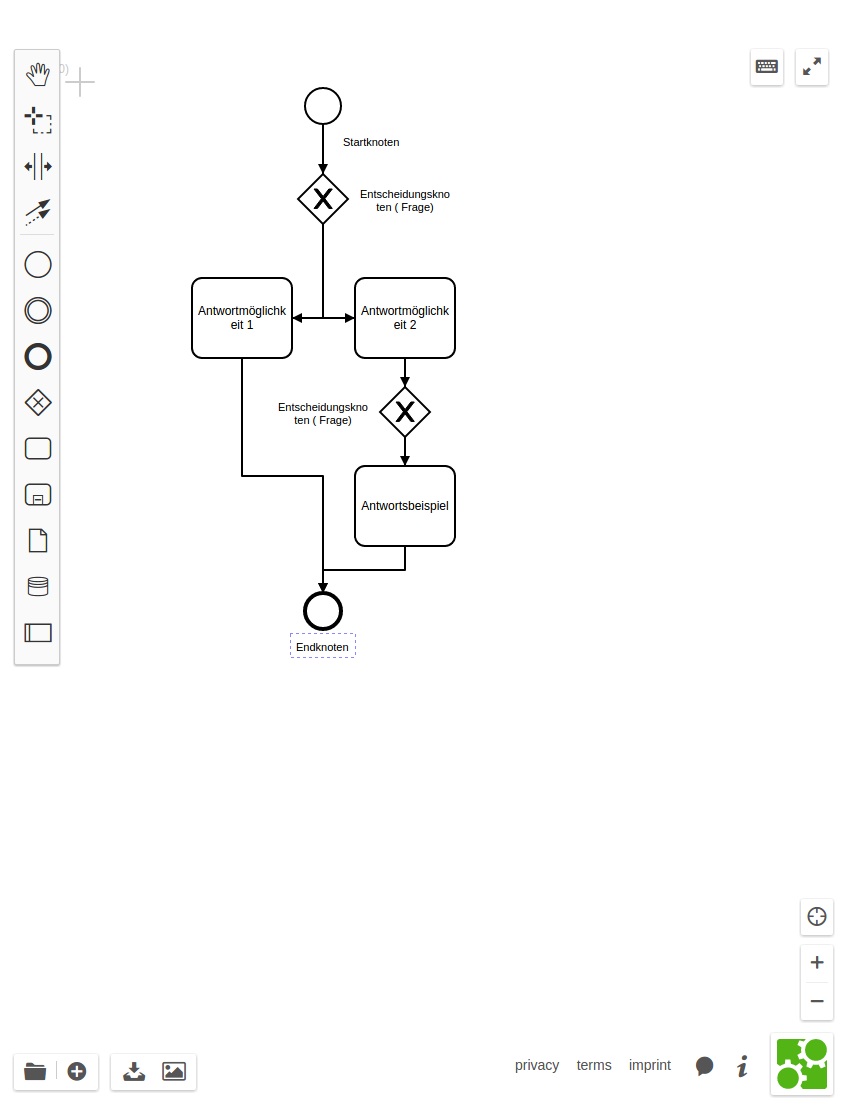
\includegraphics[scale=0.5]{images/BPMNEditorBSP}
	\caption[Screenshot des BPMN-IO Editors]{Screenshot des BPMN-IO Editors}
	\label{BPMNEditorBSP}
\end{figure}



\subsection{Aufbau der exportierten XML Datei}
Der auf diese weiße modellierte Fragebogen kann dann als XML-Datei exportiert werden. Im folgenden Abschnitt wird der Aufbau dieser Datei aufgezeigt, da im Kapitel \ref{_Implementierung} näher auf diesen Aufbau eingegangen wird. Um den Fragebogen innerhalb des Patienten Clients anzeigen zu können wird diese XML-Datei in JSON geparst

Jedes BPMN-Element im Editor, wie auch die Verbindungspfeile werden in einem XML-Element abgebildet. so wird Beispielsweise das in Abbildung \ref{BPMNEditorBSP} zu sehende \textbf{StartEvent} als \textbf{bpmn:startEvent} abgebildet. Jedes einzelne XML-Element hat eine Attribut \textbf{id} in welchem eine einzigartige Id gespeichert ist, welche aus dem Typ des Elements + einer Zufallszahl besteht. Wodurch jedes Element eindeutig identifiziert werden kann. Wurde, wie im Beispiel oben zu sehen, ein Text an das Element angehängt wird dieser in dem Attribut \textbf{name} gespeichert.

Im Fall, dass ein Verbindungspfeil(\textbf{SequenceFlow}) zwischen zwei Elementen besteht, beinhalten die XML-Elemente die Elemente \textbf{bpmn:incoming} und/oder \textbf{bpmn:outcoming}. Dessen Text spezifiziert die Id eines SequenceFlows. Dieser wird durch ein eigenes XML-Element spezifiziert. Das Element eines SequenceFlows beinhaltet immer die Attribute \textbf{sourceRef} und \textbf{targetRef}. Diese spezifizieren Anfang und Ende des Pfeils. Um nun also das Folgeelement zu einem anderen zu finden muss der ausgehende SequenceFlows gefunden werden. Das unter \textbf{targetRef} spezifizierte Element ist das Folgeelement.

Das Endelement wird durch \textbf{bpmn:endEvent} spezifiziert. Dies wurde verwendet um zu erkennen wenn der Fragebogen beendet ist.

\section{Single-Page-Application (SPA)}\label{Single-Page-Application}
Die im laufe dieser Arbeit entstandenen Clients  wurden beide als \textbf{Webanwendung (\textit{s}ingle-\textit{p}age-\textit{a}pplication)} implementiert. Sie werden zwar beide in unterschiedliche Kontexte eingebettet, basieren im Kern aber beide auf AngularJS. Eine SPA unterscheidet sich zu einer regulären Internetseite darin, dass sie nur aus einer einzelnen HTML Seite besteht. Wenn innerhalb dieser Webanwendung zu einer anderen Seite gewechselt wird, initiert dies keinen Verbindungsaufbau zum Webserver. Die Informationen über die neue Seite wurden bereits beim Seitenaufruf geladen.

Hierdurch wird der Server auf zwei Arten entlastet. Zum einen da seltener eine neue Verbindung initiiert werden muss und zum anderen weil ein Großteil der Logik auf den Client ausgelagert wird. Nach dem Laden der Hauptseite wird der Server nur noch kontaktiert um Nutzdaten zu liefern, welche jedoch auch auf einen anderen Server ausgelagert werden können.

Mit Hilfe des \textbf{Web Storage} (auch \textbf{DOM Storage} oder Supercookies genannt) ist es möglich die Daten auch auf dem Client persistent zu speichern, wodurch eine gewissen offline Funktionalität implementiert werden kann. Dies funktioniert mit SPA's besonders gut da hier Logik gespeichert wird und nicht wie im Fall einer regulären Webseite vor verarbeitete HTML Seiten. Für den Nutzer auf dem Endgerät hat diese den Vorteil, das die Seitenübergänge fließender von statten gehen, da die benötigten Daten meistens schon vorhanden sind.

\subsection{Aufbau einer SPA - Am Beispiel von AngularJS}
Hier wird kurz auf den Aufbau einer \textbf{single-page-application} eingegangen um ein grundlegendes Verständnis für die Implementierung in Kapitel \ref{_Implementierung} zu bieten.

Wie oben erwähnt besteht eine SPA nur aus einer HTML Seite, dies ist jedoch nur die halbe Wahrheit, zur besseren Übersicht werden die einzelnen Seiten der Anwendung dennoch in eigene HTML Dateien ausgelagert. Diese beinhalten jedoch ausschließlich die anzuzeigenden HTML Elemente der Seite und wird mittels AngularJS in die gewohnte \textbf{head-body} Umgebung der \textbf{index.html} eingebunden. Hierdurch wurde die in einer \textbf{Model-View-Controller Architektur} gewöhnliche \textbf{View} vom Rest der Anwendung abgekapselt. Die \textbf{Controller} werden bei \textbf{AngularJS} in eigene JavaScript Dateien ausgelagert. Diese sind für die Logik der Seite zuständig. Das \textbf{Model} beinhaltet hierbei das oben erwähnte \textbf{Web Stroage} und die Anbindung an einen Datenbank Server.

Die \textbf{index.html} ist nun also diese eine Seite die sich der Nutzer vom Server herunterlädt. Diese jedoch verlinkt die JavaScript Dateien der verwendeten \textbf{npm module} und Controllern. Ebenso werden innerhalb der \textbf{index.html} die \textbf{CSS} Dateien im Header der HTML Datei eingebunden. Anschließend wird im \textbf{Body} die Navigationsleiste spezifiziert.

Die dort verwendeten \textbf{Routen} werden in der app.js spezifiziert. Zuerst wird in dieser Datei jedoch das \textbf{angular.module} definiert, welches sozusagen als \textbf{Container} für alle anderen Teile der Anwendungen fungiert. Eine neuer \textbf{Controller} Beispielsweise, wird mittels \\ \textbf{angular.module("<moduleName">).\textit{controller}("<Name">),function("<Abhängigkeiten">)\{ "<Code"> \} );} spezifiziert und ist somit Teil des \textbf{modules}.

Die Startseite bzw. die aufgerufenen Seiten werden dann in die ebenfalls in der \textbf{index.html} definierten \textbf{ng-view} angezeigt. Jede der Seiten bzw. Routen besteht aus einer HTML Datei welche die \textbf{View} spezifiziert und einem Controller welche der Übersichtlichkeit in jeweils eigene Dateien ausgelagert sind. Im Startprojekt von Ionic werden diese in einer einzigen Datei spezifiziert.

%\todo{package.json erklären}
%\todo{Ionic - Cordova, Proxys zum Debuggen im Browser - Das CORS-Problem}
\section{Anwendungsentwicklung}\label{Anwendungsentwicklung}
Am Anfang jeder Anwendung steht die Entscheidung auf welchen Geräten diese laufen soll. Natürlich besteht die Möglichkeit eine Anwendung nativ für eine bestimmte Plattform zu entwickeln.

Um die Anwendung auf anderen Plattformen zu bringen ist es dann jedoch nötig diese praktisch neu für jede einzelne zu implementieren. Aus diesem Dilemma heraus entstanden verschiedenen Frameworks die es dem Entwickler möglich machen, direkt für mehrere Plattformen zu entwickeln. Hierdurch ist es dann möglich seinen Code nur einmal zu schreiben und diesen dann direkt, mithilfe eines Frameworks, wie zum Beispiel eines Browsers auf den verschiedene Plattformen laufen zu lassen.

Es müssen dann nur einige wenige Abschnitte des Codes nativ für die jeweilige Plattform geschrieben werden, wenn diese nicht verallgemeinerbar sind bzw. nicht schon durch eine Bibliothek vereinheitlicht wurden. Ein Beispiel wäre hier der Zugriff auf Dateien, hier ist es nicht möglich den Zugriff direkt zu verallgemeinern, da die verschiedenen Betriebssysteme unterschiedliche Dateisysteme verwenden.

Eine der Grundvoraussetzungen dieser Arbeit sollte, die Verfügbarkeit für möglichst viele Therapeuten/Patienten sein. Aus diesem Grund wurde vorab untersucht, durch welche Techniken es möglich ist, die Hürde der vielen verschiedenen Endgeräte und damit verbundenen Betriebssysteme umgehen zu können. 


\subsection{Technologie Analyse für mobile App Entwicklung}\label{MobileAnwedungsentwicklung}
Das größte Problem der Anwendungsentwicklung für Smartphones ist, dass es viele verschiedene mobile Betriebssystemen gibt. Ein kleiner Trost für jeden Entwickler ist dabei, dass sich der Hauptteil der Nutzer auf einige wenige Plattformen beschränkt. Mit einer Anwendung für Android, IOS und Windows kann man somit den größten Teil der Nutzer erreichen. Diese decken über 99\% \cite{STA16} der Smartphone Benutzer ab.

 
\subsubsection{Plattform spezifische Entwicklung}
Durch die nativen Anwendungsentwicklung wird eine mobile Anwendung nur jeweils für eine Plattform entwickelt. Hierdurch hat man aber den Vorteil, dass man durch wegfallen jegliches Frameworks die maximale Geschwindigkeit und minimale Reaktionszeiten erzielt.

Dies ist vor allem wichtig bei rechenintensiven Anwendungen wie Spielen oder ähnlichem. Des weiteren hat man durch die native Entwicklung den vollen Zugriff auf jegliche im Smartphone verbaute Hardware und Betriebssystem Features. Bei Verwendung eines Frameworks müssen hier oft Abstriche gemacht werden.

\subsubsection{Cross Plattform Entwicklung}
Von Cross Plattform Entwicklung spricht man, wenn der Code der entwickelten Anwendung nicht nur für eine spezifische Plattform verwendbar ist. Durch verschiedene Frameworks ist es möglich, dass der Entwickler die Anwendung nur einmal schreibt und diese dann auf den meist verwendeten Betriebssystemen läuft oder für diese übersetzt wird. Dies wird Grundlegend auf \textbf{3 verschiedenen} Wegen erreicht.

\paragraph{Web-Apps / Webanwendungen}laufen im vom Betriebssystem zur Verfügung gestellten Webbrowser. Hierbei ist das Betriebssystem völlig egal. Es werden nur einige Voraussetzungen an den Webbrowser gestellt, welche jedoch von dem meisten neuer Browsern erfüllt werden.

Ebenso wird eine aktive Internetverbindung benötigt wenn die App ausschließlich online zur Verfügung steht. Um dies zu umgehen wurde in HTML5 verschiedenen Möglichkeiten eingebaut um Code und Daten lokal zwischenspeichern zu können. Dadurch, dass die App auf eine Webserver gehostet ist, kann diese schnell veröffentlicht und aktualisiert werden. Wenn der Nutzer die Anwendung mit einer aktiven Internet Verbindung öffnet, aktualisiert sich die App automatisch. 

\begin{figure}[H]
	\centering
	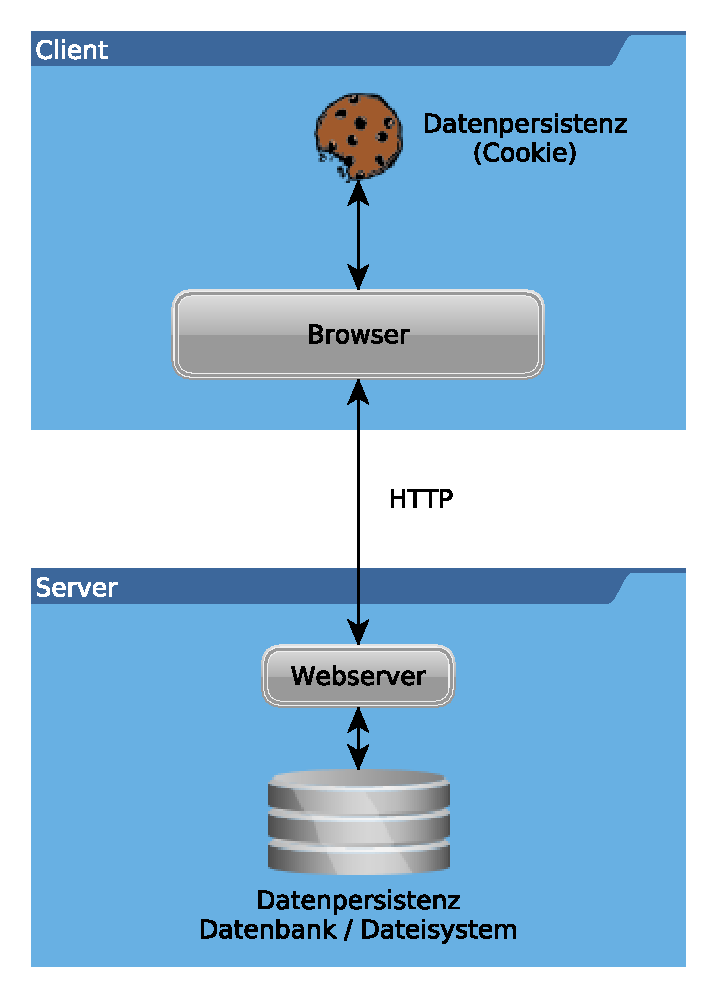
\includegraphics[scale=0.8]{images/Webapps}
	\caption[Schematische Darstellung einer WebApp]{Schematische Darstellung einer WebApp}
	\label{Webapps}
\end{figure}

Sofern es sich bei der Anwendung nicht um eine sogenannte \textbf{Single Page Application} handelt, wodurch die Berechnungen auf den Client ausgelagert werden würden, übernimmt der Server, welcher die Anwendung hostet einen Großteil der Datenverarbeitung. Dann dient der Client lediglich der Anzeige der Anwendung und Interaktion mit dem Nutzer.

Der Nachteil dadurch das die App im Webbrowser läuft ist, dass man nur Zugriff auf die Funktionen hat, die der verwendete Browser bietet. Da ein Webbrowser nicht zwangsläufig auf einem mobilen Gerät mit diversen Sensoren laufen muss, ist der Zugriff auf die gängigen Sensoren in einem mobilen Endgerät meist sehr eingeschränkt. Auf Grund dessen muss man sich bei der Web-App Entwicklung meist auf Kamera, Datenpersistenz und GPS beschränken.

Durch die Zentralisierung der App sieht diese auf jedem Gerät gleich aus. Dies erscheint im ersten Augenblick positiv, der Benutzer jedoch ist an das Bedienkonzept seines Betriebssystems gewohnt, wodurch Apps welche nicht auf das Betriebssystem zugeschnitten sind meist keinen sehr großen Anklang bei den Nutzern findet. 

\paragraph{Hybride Apps}\label{Hybride Apps} basieren wie auch die Web-Apps auf den Webtechnologien HTML5, CSS und JavaScript. Laufen aber im Gegensatz zu dem Web-Apps in einem mitgelieferten Minibrowser(Webview Container) oder, für den Nutzer nicht sichtbar, im vom Betriebssystem bereitgestellten Webbrowser. Dann werden jedoch jegliche Bedienelemente, wie Beispielsweise die URL-Leiste oder sonstige Buttons durch das Framework ausgeblendet.

\begin{figure}[H]
	\centering
	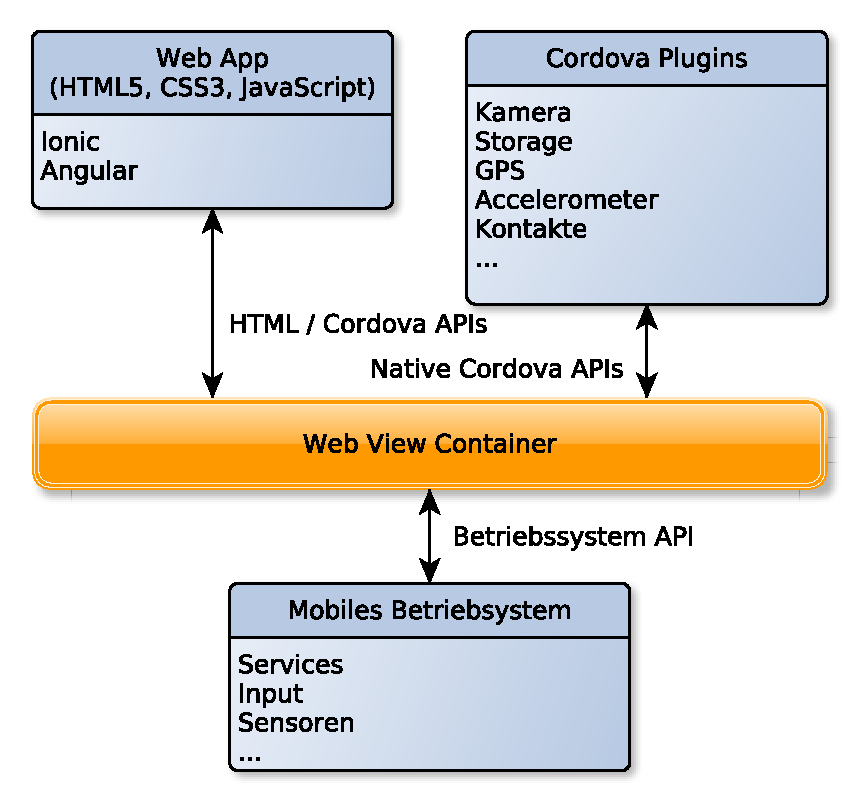
\includegraphics[scale=0.8]{images/IonicCordova}
	\caption[Aufbau des Ionic-Cordova Frameworks]{Aufbau des Ionic-Cordova Frameworks}
	\label{IonicCordova}
\end{figure}

Dieser Container ist in einer nativen App eingebettet was den Zugriff auf die System APIs des Geräts erlaubt. Durch das einbetten von nativen Code ist der Zugriff auf alle vom Betriebssystem zur Verfügung gestellten Funktionen möglich. wie z.b. GPS, Kamera, Betriebssystembenachrichtigungen und die verschiedenen Sensoren(Beschleunigung, Umgebungslicht, Hall, Gyroskop,...). 

Da die Anwendung im Herzen eine Internetseite ist, ist es implizit möglich diese unter einer URL zu veröffentlichen und wie eine Web-App zu behandeln. Dann jedoch auch mit den Einschränkungen die diese bietet.

Für den Entwickler sehr angenehm sind oft angebotene "<Live-View"> Technologien. Diese erlauben durch speichern einer HTML oder JavaScript Projektdatei ein neu laden der App im Webbrowser zu initiieren. Dies bietet ein schnelles Designen der Oberfläche und implementieren grundlegender Funktionen. Systemeigene Funktionen müssen jedoch auf einem Gerät oder im Emulator getestet werden. Hierzu ist dann compilieren, packen und ausliefern notwendig, was etwas Zeit benötigt.
\newpage
\paragraph{Native Cross Plattform Apps} mit gemeinsamer Codebasis verspricht \textbf{Xamarin}, ein Projekt das auf der quellen-offenen Implementierung von Microsofts .NET Framework, Mono basiert \cite{MONO16}. Mittels des Mono Frameworks ist es möglich C\# Code auf verschiedenen Betriebssystemen laufen zu lassen. Der geschriebene Code wird dann beim Bauvorgang der App in Nativen Code umgesetzt. Es fällt somit im Gegensatz zu den Hybriden Apps, das Framework auf dem Endgerät weg, wodurch Rechenkapazität gespart wird. Was diese Plattform vor allem für rechenintensivere Anwendungen interessant macht.

\begin{figure}[H]
	\centering
	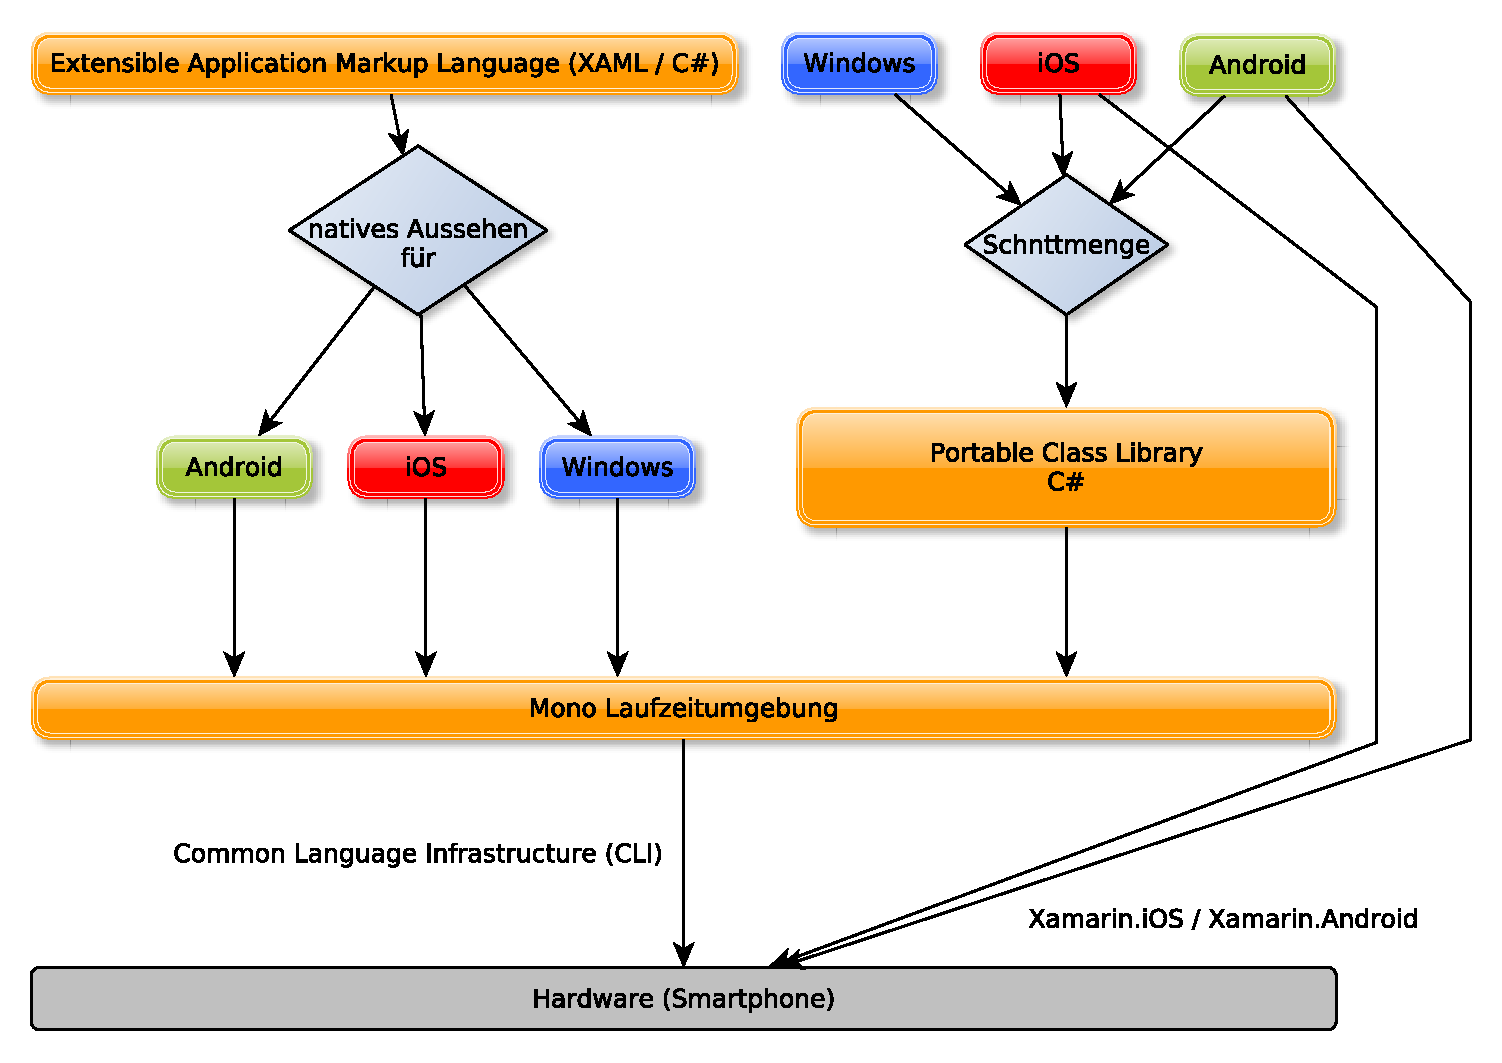
\includegraphics[scale=0.58]{images/Xamarin}
	\caption[Aufbau des Xamarin Frameworks]{Aufbau des Xamarin Frameworks}
	\label{XamarinBild}
\end{figure}

Bei der Erstellung einer Cross Plattform App mittels Xamarin muss man zuerst festlegen, auf welchen Betriebssystemen diese später laufen soll. Aus dieser Auswahl wird eine Schnittmenge der Funktionen gebildet die zur Verfügung stehen und eine sogenannte \textbf{Portable Class Library} erzeugt. Diese fungiert dann als einheitliche Schnittstelle bei API aufrufen an das Betriebssystem.

Es sind jedoch nur die Funktionen Plattform übergreifend nutzbar, welche von allen ausgewählten Betriebssystemen angeboten werden und von Mono implementiert sind. 
Sollte der Entwickler Zugriff auf systemeigene Funktionen benötigen, welche nicht von Mono abgedeckt werden, hat er mit Xamarin.iOS und Xamarin.Android die Möglichkeit alle systemeigenen Funktionen verwenden zu können. Zur Vereinheitlichung unter einer gemeinsamen GUI ist es dann aber nötig die Funktion für jedes Betriebssystem separat zu entwickeln und zu pflegen.

Mittels Xamarin.Forms ist es möglich die GUI der App Plattform übergreifend zu gestalten. Hierzu wird die Oberfläche mittels einer eigenen, XML ähnlichen, Sprache namens \textbf{Extensible Application Markup Language (kurz XAML)} beschrieben. Die so spezifizierten Views werden dann auf die einzelnen Betriebssysteme zugeschnitten, um dem Anwender eine gewohnte Umgebung zu bieten. 

\section{Software Analyse} \todo{vielleicht noch Tabellen der Vorteile aller}
Im folgenden Kapitel soll untersucht werden mit Hilfe welcher Technologien die Plattform realisiert werden kann. Hierbei wird eine Abwägung getroffen, welche Vor- und Nachteile die einzelnen Technologien mit sich bringen. Zuerst werden Technologien für den Desktop Client des Therapeuten untersucht. Anschließend wird die Entwicklung einer mobilen Anwendung für den Patienten Client untersucht.

\subsection{Therapeuten Client}
Der Therapeuten Client sollte eine Desktop Anwendung sein. Diese benötigt keine intensive Rechenkapazität, Grafikleistung oder dergleichen.
Genau dies wären jedoch die Vorteile der nativen Entwicklung, neben der näheren Anbindung von Peripheriegeräten. Da aber auch diese für die Anwendung nicht von Nöten sind, wird untersucht, mit Hilfe welcher Technologien eine möglichst breites Feld an Endgeräten abgedeckt werden kann.

Hierfür gibt es sehr viele unterschiedliche Plattformen und Frameworks welche auf völlig unterschiedlichen Technologien aufbauen. Was alle gemeinsam haben, ist eine Laufzeitumgebung in welcher das entwickelte Programm später läuft. Eine der bekanntesten ist hier wohl Java aber auch Mono, die quellen-offene Implementierung von Microsofts .NET Framework sollte hier nicht außer acht gelassen werden. 

Des weiteren gibt es wie auch für die mobile Cross-Plattform-Entwicklung Frameworks, welche einen Mini Browser bereit stellen welcher die Anzeige und Interaktion verwaltet. Die eigentliche Anwendung ist eine \textbf{single-page-application}, welche zusammen mit dem Mini Browser, sozusagen in diesen integriert, ausgeliefert wird. Ein Beispiel für diese Technologie ist das TideSDK mit dessen Hilfe Webentwickler Anwendungen für Windows, Mac OS X und Linux entwickeln können.

Eine weitere Anforderung an die zu entwickelnden Plattform ist die globale Persistenz der Daten über beide Clients. Diese Anforderung wurde mittels eines Webservers gelöst. Aus diesem Umstand heraus wurde beschlossen, den Client für den Therapeuten in Form einer \textbf{single-page-application} [\ref{Single-Page-Application}] zu implementieren, da diese auf jedem Geräten mit aktuellem Browser angezeigt werden kann und auf dem selben Server wie die Datenpersistenz gehostet werden kann.
Hierdurch ist es dem Therapeuten auch möglich die Anwendung auf einem Tablet oder Handy zu öffnen, ohne diese installieren zu müssen.

\subsection{Patienten Client}
Der Patienten Client sollte eine App für mobile Endgeräte sein, da der Patient dann einfach an die Erledigung  seiner Übung erinnert werden kann. Abgesehen davon bietet ein Smartphone viele Sensoren, welche zur Unterstützung der Therapie hilfreich sein können. Um möglichst viele Patienten mit dieser Anwendung erreichen zu können, wurde beschlossen diese nicht nativ nur für eine Plattform zu entwickeln. In Tabelle \ref{VorteileNativ} sind die Vorteile der nativen App Entwicklung aufgezeigt.

\begin{table} [H]
	\begin{center}
		\begin{tabular}{p{4cm} p{10cm}}
			\rowcolor{black!20}  \textbf{Vorteil} & \textbf{Beschreibung} \\
			\hline \toprule
			maximale Performance & nativer Code, dadurch keine Laufzeitumgebung nötig die Multi-Plattform-Code interpretiert \\ \hline \addlinespace
			geringere Reaktionszeiten & direktes ansprechen von Geräte API, Prozessor und Speicher \\ \hline \addlinespace
			Keine Beschränkung durch Laufzeitumgebung & Keine Laufzeitumgebung die den Entwickler auf die gebotene API einschränkt \\ \hline \addlinespace
		\end{tabular}
	\end{center}
	\label{VorteileNativ}
	\caption[Vorteile der nativen App Entwicklung]{Vorteile der nativen App Entwicklung}
\end{table}

Es gibt viele Plattformen welche es erlauben, gleichzeitig für mehrere mobile Betriebssysteme zu entwickeln. Hier sollen einige dieser Plattformen und Frameworks genannt sowie deren Vor- und Nachteile aufgezeigt werden.

\subsubsection{Ionic}
Ionic ist ein Open-Source-Framework welches es erlaubt den geschriebenen Quellcode plattformübergreifend zu verwenden. Das Framework basiert auf Apache Cordova und AngularJS und wird mittels der Webtechnologien HTML, CSS und JavaScript geschrieben. AngularJS liefert die Grundstruktur der App, auf die später in diesem Kapitel noch genauer eingegangen wird.

Cordova liefert hierbei die Laufzeitumgebung der App, wodurch diese in einer mitgelieferten, nativen \textbf{WebView} auf dem Gerät angezeigt wird. Dieser WebView-Container bietet im Gegensatz zum nativen Browser den Vorteil, dass durch ihn die nativen APIs des Gerätes angesprochen werden können. Hierdurch ist es möglich auf alle Fähigkeiten wie Benachrichtigungen, Kamera, Speicher, Kontakte,... des Gerätes zuzugreifen.

Ionic selbst kümmert sich vor allem darum, dass sich die App auf jedem Endgerät nativ anfühlt, es werden alle Elemente an die Betriebssystem Richtlinien angepasst. Sowohl das Aussehen als auch die Platzierung, Beispielsweise des Zurück-Buttons oder des Kontext Menüs, wird angepasst, je nachdem für welche Plattform die App gebaut wird. 

Des weiteren bietet Ionic verschiedene Mechanismen, welche die Entwicklung angenehmer machen. Mittels des \textbf{Ionic Creator}s kann die App im Browser oder in einer mitgelieferten GUI direkt auf \textit{quasi emulierten} Geräten getestet werden. Durch das sogenannte \textbf{live reload} wird die App ob nun im Browser oder auf dem Gerät laufend neu geladen, wenn eine Codeänderung vorgenommen wurde.


\subsubsection{Xamarin}
Der größte Vorteil von Xamarin bei der Cross-Plattform-Entwicklung ist die Performance. Während hybride App eine  schlechtere Performance gegenüber native Entwickelten Apps haben schafft es Xamarin, dadurch dass es nativen Code generiert, teilweise sogar eine bessere Performance an den Tag zu legen wie mit \textbf{Objective-C} programmierte iOS Apps \cite{WINUNIT16}. Auch im Vergleich mit nativ entwickelten Anwendungen für Android schneidet Xamarin sehr gut bis hin zu besser ab \cite{MEDIUM16}. Nur Apps welche in C++ entwickelt wurden sind sowohl auf iOS als auch auf Android absoluter Spitzenreiter wenn es um die Performance geht.

Dadurch, dass Xamarin nativen Code erzeugt es nach einer Änderung im Quellcode jedes mal bevor man diese sichtbar machen kann nötig die App zu bauen und auf ein Gerät oder in den Emulator auszuliefern, was jedes mal relativ viel Zeit in Anspruch nimmt. Eine \textbf{live-view} Funktion wie es Ionic anbietet gibt es auf dieser Plattform nicht.

Einer der größten Nachteile von Xamarin ist der Preis. Wobei es seit einiger Zeit eine kostenlose Version gibt, welche für Forschung, Open Source Projekte sowie Bildung und kleine Teams verwendet werden kann. Wenn man mit einer solchen App Geld verdienen möchte, will Xamarin auch etwas davon haben.




